\newpage
\thispagestyle{sectioned}
\chapter{Metodología del Proyecto}

\section{Uso de Software Libre}

\section{Metodología de Migración de Wave a Android}

\section{Diseño de la Aplicación: Diseño Guiado Por Objetivos}

Para elaborar el diseño de la aplicación, nos hemos basado en la metodología del Diseño Guiado por Objetivos, que implementa el proceso de la Ingeniería de la Usabilidad propuesto por Alan Cooper \cite{ref:bookAlanCooper}. Este proceso constará de las siguientes fases:

\begin{itemize}
	\item \textbf{1. Investigación}
	\item \textbf{2. Modelado}
	\item \textbf{3. Definición de Requisitos}
	\item \textbf{4. Framework de Diseño}
\end{itemize}

Queremos insistir eso sí en que únicamente nos hemos basado en esta metodología para seguir el proceso del diseño de la aplicación. No seguiremos todas las fases de esta metodología al pie de la letra ya que el alcance en tiempo de este proyecto escapa a una metodología tan formal y laboriosa (que implica gran cantidad de pruebas y procesos) como esta.

\subsection{Investigación}

\subsubsection{Intención Inicial: Prototipo básico}  

¿HABLAR DE INTENCION FUTURA PARA ELECCIONES?

Programas electorales

La intención fundamental de la aplicación es llevar los programas electorales a los bolsillos de los ciudadanos y generar interés en participar más activamente en la política, ya sea emitiendo opiniones sobre dichos programas o elaborando nuevas propuestas. Vivimos en una sociedad digital, donde cada vez son más las personas que utilizan sus smartphones para realizar todo tipo de tareas en su vida cotidiana.

En los últimos años las diferentes formaciones políticas han subido sus programas electorales a un documento en formato PDF que suele estar disponible para su descarga en su página web. Este documento tiene generalmente una gran extensión (los hay de 200 páginas), lo cual no hace sino dificultar que las personas se animen a leerlo. Por ello pensamos que una aplicación que pudiera visualizar las principales secciones de los programas políticos podría ser especialmente útil para acercar los programas a los electores.

Además también intentariamos darle una estructura a estos programas, de manera que el usuario pudiera navegar por ellos a nivel de Sección, a diferencia del método actual de leer un "macro-documento" en PDF. Así, la gente podría opinar sobre los programas políticos a nivel de sección mediante acciones familiares para ellos: "Me gusta", "No me gusta" y realizar "Comentarios". Añadimos también una acción de "No lo entiendo" que pensamos que seria util para indicar cuándo la redacción de la sección era de significado difuso.

En definitiva, queríamos crear un espacio donde poder informarse sobre las distintas ofertas electorales y poder debatir sobre las propuestas que propone cada formación política, todo ello en forma una aplicación que podremos consultar en cualquier momento. 

Propuestas y Wave

Por otro lado,y en línea con los últimos movimientos políticos ciudadanos, pretendíamos crear también un portal de propuestas ciudadanas en el móvil. Los usuarios podrían visualizar las propuestas de otros usuarios y tener la posibilidad de crear nuevas propuestas. Además, como queríamos aprovechar las características de la migración de Wave previamente desarrollada, pensamos en la posibilidad de elaborar estas propuestas de forma colaborativa y en tiempo real entre muchos usuarios.

Actualmente existen multitud de portales (en su gran mayoría web) donde la ciudadanía puede expresar su opinión, pero creemos que la integración de una aplicación donde puedan situarse las opiniones de los partidos políticos (en forma de sus programas) y la actividad ciudadana (en forma de propuestas), genera una nueva manera de tratar la política en los medios sociales.

También pensamos en la posibilidad de categorizar el contenido de la aplicación (Programas y Propuestas) por temas, para proporcionar filtros a la hora de navegar por dicho contenido. Sin embargo no teníamos muy clara la elección de temas, asi como si debiamos darle al usuario la posibilidad de crear nuevos temas o dar nosotros unos temas preestablecidos.
 
Una vez pensada la intención y los principales objetivos de la aplicación, procedimos a realizar unos primeros prototipos en papel de nuestra idea y a implementar un prototipo básico en el móvil (Ver Sección \ref{ssec:prototypes}) que mostraba programas políticos estructurados y permitía navegar a nivel de Sección por ellos para leer y emitir opiniones (likes, dislikes, comentarios, etc.).  

 El siguiente paso sería estudiar la viabilidad de esta aplicación entrevistando gente para realizar una investigación sobre sus necesidades prácticas. Por otra parte también sería útil enseñarles los prototipos básicos que manejábamos para verificarlos. Entendimos que el tipo de persona con el que nos entrevistáramos debía de estar relacionado de alguna manera con el mundo de la política, pues nada mejor que hablar con gente ya interesada en dichos temas para orientarnos por el buen camino.

A continuación detallamos las entrevistas que realizamos en la investigación:

\subsubsection{Entrevista con Labodemo}

Tuvimos la oportunidad de mantener una conversación con dos miembros de Labodemo \cite{ref:labodemo}, en la que aprovechamos para mostrarles un prototipo de la aplicación que estábamos desarrollando. Ambos tenían experiencia en el desarrollo de plataformas de participación ciudadana en Internet: fueron los responsables del desarrollo de los portales de participación del partido político Podemos y la candidatura ciudadana de unidad popular Ahora Madrid.

En ese momento nuestro prototipo móvil se limitaba únicamente a mostrar las diferentes secciones de cada programa, lo cual les pareció útil, aunque no lo suficiente como para atraer a una cantidad considerable de usuarios. Conforme a su linea de trabajo habitual, eran más partidarios de dar a los usuarios la posibilidad de realizar Propuestas además de ver Programas políticos. Les comentamos entonces que antes de hablar con ellos ya habíamos planteado desarrollar Propuestas colaborativas en tiempo real aprovechando la tecnología de Wave. Pero ellos no eran partidarios de esta opción, ya que según ellos acabaría siendo caótico tener tanta gente editando la misma propuesta de cara a generar contenido útil. 

Dándole una vuelta a la categorización del contenido, nos sugirieron que para atraer a usuarios, debíamos considerar la posibilidad de integrar en la aplicación a colectivos sociales que generaran y categorizaran dicho contenido. No eran partidarios de que dieramos nosotros ciertas temáticas preestablecidas, pues debido a la variedad de redaccion en los distintos programas sería dificil identificar temáticas que incluyeran a todos los programas y probablemente acabariamos excluyendo temas. Así, serían los colectivos los que se encargaran de "tematizar" el contenido de la aplicación. Por ejemplo: un grupo de animalistas podría tener un espacio en la aplicación donde poder crear sus propias propuestas, e incluso hacer comparativas de lo que proponen los diferentes programas sobre los animales. 

De esta manera, y en relación a la aproximación a los foros tradicionales, se planteó la idea de crear "Hilos": elementos "temáticos" que agruparan en un solo sitio Secciones y Propuestas que hablaran sobre un determinado tema. Estos hilos serían también generados por dichos colectivos.

Esto sería útil también para usuarios que buscaran información sobre un determinado tema. Por ejemplo: un usuario poco activo, que resulta ser profesor, podría buscar un colectivo de profesores y ver las Propuestas que se llevan a cabo o visualizar una comparativa respecto las medidas de educación de los diferentes programas políticos.

Nos insistieron mucho en el tema de las comparativas. Sería de gran utilidad que la aplicación tuviera una parte de comparativas en la que los usuarios pudieran comparar los programas políticos en vez de leerlos sección por sección. Resultaría de gran interés a un autónomo visualizar las medidas que proponen los diferentes partidos políticos para los autónomos. Pero estas comparativas no podría realizarlas cualquiera, por lo que deberían realizarlas periodistas o expertos que hubieran realizado algún tipo de comparativa similar anteriormente. Nos sugirieron contactar con periodistas o colectivos que hubieran publicado algún tipo de comparativa en cuanto a programas o medidas, para obtener algún tipo de ayuda o consejo a seguir.

\subsubsection{Conclusión}

¿PROTOTIPOS? 

La reunión con dos de los miembros de Labodemo resultó de gran interés. Se trataba de personas que tenían mucha experiencia en desarrollo de portales de participación ciudadana y que sobre todo estaban muy familiarizados con el uso común que le suele dar la gente a este tipo de aplicaciones. A priori, sabían mejor que nosotros cómo determinar las claves para que una aplicación tuviera una aceptación y uso considerable de los usuarios desde el principio.

Visualizar los programas políticos en la app no les entusiasmó demasiado. Expusieron que, a priori, un ciudadano de a pie no iba a molestarse en meterse en la aplicación para leer los programas políticos de los diversos partidos. Ellos argumentaban que los colectivos sociales serían los usuarios más activos en nuestra aplicación, por lo que debíamos enfocar más el desarrollo hacia la participación ciudadana y la generación de Propuestas o Comparativas de Secciones de Programas hechas por tales colectivos. Dichas Comparativas sí que generarían más interés por leer los programas políticos.

Tras la reunión tomamos nota de los consejos que obtuvimos de Labodemo. Incluimos la idea de "Comparativas" y empezamos a pensar la forma de colaborar de grupos y colectivos. También intentamos contactar con colectivos y personas interesadas en el desarrollo de la aplicación. 

Finalmente, conseguimos concretar una entrevista con Javier de la Cueva \cite{ref:jdelacueva}.

\subsubsection{Entrevista con Javier de la Cueva}

La entrevista con Javier de la Cueva resultó bastante productiva. Ya le conocíamos de algunas conferencias que impartió en la facultad. Javier es abogado y doctorado en Filosofía, estando especializado en temas relacionados con tecnología, Internet y propiedad intelectual. Además, en sus últimas conferencias Javier habla sobre acciones micropolíticas \cite{ref:manualCiberactivista}. Estas acciones definen la capacidad que tienen los ciudadanos para realizar aportaciones a la sociedad, el estado o el gobierno que favorezcan la participación ciudadana en una democracia participativa.

Representar los programas electorales en una aplicación móvil le pareció algo interesante y necesario para la sociedad actual. Si bien casi nadie hace el esfuerzo de visualizar un programa electoral en PDF, utilizar una herramienta que facilita el acceso al programa por secciones podría ser una nueva forma de incentivar su lectura y ayudar a fomentar la participación ciudadana en política. 

Además nos sugirió la posibilidad de desarrollar una Hemeroteca de programas electorales. De esta forma cualquiera podría consultar los programas de los anteriores gobiernos y comprobar si se cumplieron los objetivos del programa, así como comparar programas de distintos años entre sí, 

Pero si en algo nos insistió Javier, fue en la importancia de categorizar el contenido de la aplicación. Un usuario que no tenga conocimientos sobre diversos temas, se encontraría más cómodo si pudiera visualizar las diferentes partes de un programa o las propuestas ciudadanas por categorías o temas generales. Ya que dejar libertad a los usuarios para crear categorías personalizadas podría ser algo negativo para usuarios inexpertos o con pocos conocimientos sobre temas específicos.

Por último, centrándonos en las Propuestas ciudadanas, surgió la idea de elaborar propuestas que tuvieran una especificación concreta. Es decir, a parte de tener una idea de propuesta y redactarla, esta propuesta debería ir acompañada de los recursos que serían necesarios y sobre todo cómo se llevaría a cabo de una forma aproximada. También resultaría interesante definir un pequeño presupuesto de lo que conllevaría realizar la propuesta o cómo se podría financiar. Así evitaríamos una elaboración de propuestas más real, evitando un listado de propuestas infinito sin planterase cómo se llevarían a cabo o cómo se financiarían.

\subsubsection{Conclusión}

Javier trató de abrirnos un poco más la mente, para plantearnos ideas que no están representadas en la sociedad. En la actualidad encontramos diversas plataformas de participación ciudadana que acaban convirtiéndose en un foro. Para evitar caer en esto, debíamos innovar algo más para volver a repetir esto, debíamos de intentar desarrollar nuevas formas de participación.

Clasificar las secciones de un programa así como también las propuestas ciudadanas en diferentes categorías y temas era algo que descartamos en un principio, pero nuevamente volvió a llamar nuestro interés. Aunque para dar cierta libertad, podríamos incluir la posibilidad de crear categorías personalizadas o ir añadiendo categorías semanalmente.

\subsection{Modelado}

En esta fase definiremos el tipo de persona que interactuará con nuestra aplicación. Para ello hemos identificado dos tipos de personas primarias:

\textbf{- Activista social, 16 años en adelante}

\underline{Actividad:}

\begin{itemize}
\item Estudia, trabaja o realiza otras actividades de voluntariado.
\item Frecuenta asambleas, participa en diferentes movimientos sociales y está al día de la actualidad política.
\item Utiliza redes sociales para comunicarse con otros colectivos, acudir a asambleas, promover ideas u otras actividades relacionadas con la política y el activismo social.
\end{itemize}

\underline{Otros:}

\begin{itemize}
\item Desconoce las ideas que proponen algunos partidos 
\item Le gusta aportar nuevas soluciones a la sociedad.
\end{itemize}

\textbf{- Ciudadano de a pie, 18 años en adelante}

\underline{Actividad:}

\begin{itemize}
\item Estudia, trabaja o realiza otras actividades de voluntariado.
\item Es distante al mundo de la política, concibe ciertos temas pero no los conoce en profundidad.
\item Visita diferentes medios de comunicación para enterase de la actualidad.
\item Utiliza redes sociales para compartir contenidos con sus amigos o establecer nuevas amistades.
\end{itemize}

\underline{Otros:}

\begin{itemize}
\item Desconoce por completo los programas electorales. 
\item Tiene cierta indecisión a la hora de acudir a las urnas, no sabe que propone cada partido.
\end{itemize}

\subsection{Definición de Requisitos}

En esta sección se definirán los posibles escenarios que puedan surgir en la aplicación:

\textbf{Escenario I}

Se acercan las elecciones municipales y Juan aún no ha decidido a qué partido va dar su voto. No conoce las propuestas que ofertan los partidos a la ciudadanía y tampoco se fía mucho de lo que dicen los medios de comunicación.

Juan coge su móvil y visualiza los diferentes programas electorales por categoría, seleccionando la categoría de educación que es la que más le afecta a él personalmente. La aplicación le muestra un listado de las secciones donde lso diferentes partidos hablan de las medidas que van a tomar en torno a la educación.

\underline{Requisitos:}

\begin{enumerate}
\item Visualizar (acción) las diferentes categorías (objeto), para ver las secciones de los programas de una determinada categoría (contexto).
\item Mostrar(acción) un listado de todas las secciones de los programas de los partidos  políticos (objeto) en función de la categoría seleccionada por el usuario (contexto).
\end{enumerate}

\textbf{Escenario II}

Pablo es un empleado sanitario de Hospital Clínico de Madrid preocupado por la gestión de los hospitales públicos. Parece que la situación no está muy controlada, por lo que quisiera saber que propuestas o alternativas propone la ciudadanía para mejorar la situación actual.

A través de su móvil puede explorar las diferentes propuestas por categorías. Eligiendo la categoría de sanidad, le aparece un listado de las últimas propuestas desarrolladas por la ciudadanía.

\underline{Requisitos:}

\begin{enumerate}
\item Mostrar (acción) las diferentes categorías (objeto), para visualizar las propuestas ordenadas por la categoría seleccionada (contexto).
\item Visualizar (acción) el listado de propuestas (objeto), clasificados por la categoría seleccionada por el usuario (contexto).
\end{enumerate}

\textbf{Escenario III}

\underline{Requisitos:}

\begin{enumerate}
\item
\item
\item
\end{enumerate}

\textbf{Escenario IV}

\underline{Requisitos:}

\begin{enumerate}
\item
\item
\item
\end{enumerate}

\textbf{Escenario V}

\underline{Requisitos:}

\begin{enumerate}
\item
\item
\item
\end{enumerate}

\subsection{Framework de diseño} \label{ssec:prototypes}

En esta sección detallaremos todos los aspectos relacionados con el aspecto visual de la aplicación. Detallaremos los prototipos desarrollados en papel, algunos prototipos intermedios y el prototipo final de la aplicación.

\subsubsection{Metodología} 

En una primera fase procedimos a realizar una serie de prototipos rápidos a papel para visualizar una interacción de las principales características de la aplicación. A continuación llevamos estas ideas en papel a nuestra aplicación desarrollada en Android. Obteniendo un prototipo de media-alta fidelidad sobre la funcionalidad de la aplicación. Este fue el prototipo que enseñamos en las entrevistas durante la fase de investigación.

Cuando quisimos añadir nuevas características tras sacar conclusiones de las entrevistas, volvimos a desarrollar nuevos prototipos en papel de las pantallas a desarrollar. Por último, se desarrollaron las nuevas pantallas y se refinaron las anteriores para llegar a un prototipo de alta fidelidad o una versión alpha de la aplicación.

\subsubsection{Prototipos en papel}

Meter las fotos de los prototipos en papel y comentarlos.

\subsubsection{Prototipos intermedios}

La aplicación pretende llevar las principales partes de los programas electorales de los partidos que se presenten a las elecciones. Por tanto, cualquier usuario podrá visualizar el apartado que desee consultar de cualquier partido político. Siendo esta la forma menos amigable de leerlo, se utilizarán distintas formas para compartir o divulgar determinadas secciones más populares.

Al inicio de la aplcación, mostrará una lista de las secciones de los programas más valoradas, más debatidas, peor valoradas e incluso las más incomprendidas. Por tanto creemos que puede ser una forma de acercar aquellas secciones más populares de forma más eficaz, al contrario que tener que consultar una determinada página dentro de un extenso pdf.

\begin{figure}[H]
\centering
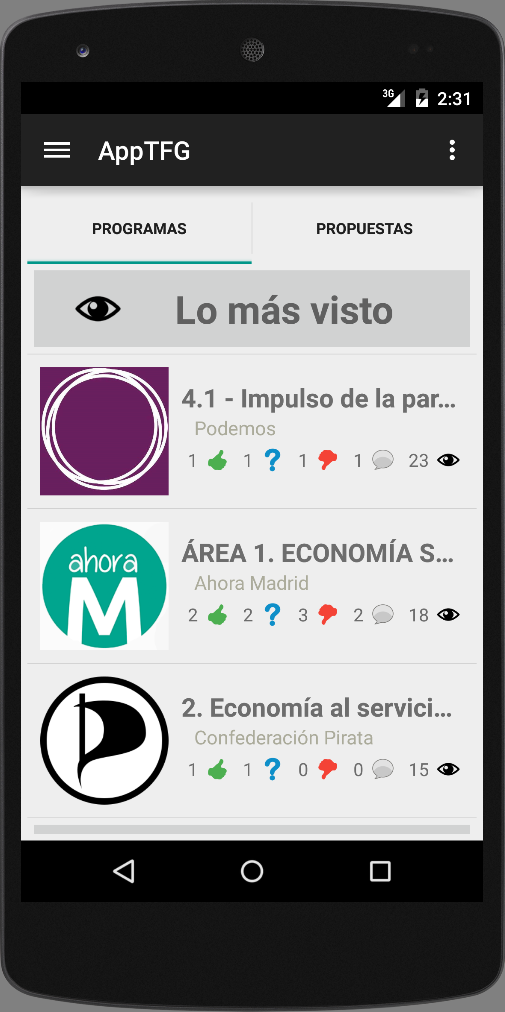
\includegraphics[keepaspectratio, scale=0.5]{Media/Captures/captTopSections.png}
\caption{Vista principal de secciones}
\label{fig:captTopSections}
\end{figure}

Dentro de cada sección podemos visualizar el contenido de la sección a la que referencia el programa, y tendremos la opción de valorarla de forma positiva o negativa. También añadimos la posibilidad de indicar que no se ha entendido la sección. Pues a la hora de leer una propuesta de gobierno ubicada en una sección del programa, bien nos puede gustar, disgustar o simplemente no haber entendido la idea y por ello no votarla de forma positiva o negativa.

\begin{figure}[H]
\centering
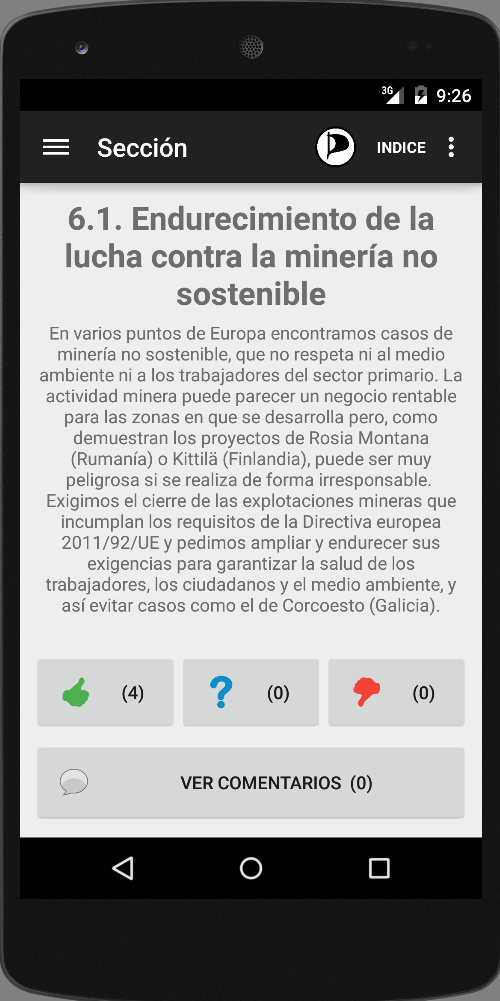
\includegraphics[keepaspectratio, scale=0.5]{Media/Captures/section.png}
\caption{Visualizando una sección}
\label{fig:captSection}
\end{figure}

Sin olvidarnos de la parte social, en cada sección podemos hacer comentarios para intentar debatir las ideas fundamentales que propone la sección. O incluso hacer referencia a una determinada frase o párrafo.

\subsubsection{Prototipo final}

\subsection{Análisis de Usabilidad}

Hablar de las reglas de oro, principios de diseño,...

\section{Implementación de DemoCritics}

\section{Evaluación con Usuarios}

